\documentclass[12pt]{scrartcl}

 

\usepackage[utf8]{inputenc}

\usepackage[T1]{fontenc}

\usepackage{lmodern}

\usepackage[ngerman]{babel}

\usepackage{amsmath}

\usepackage{graphicx}


 

\title{Versuch E3\\ Elektronen im elektrischen und magnetischen Feld}

\author{Frederik Strothmann, Henrik Jürgens}

\date{\today}


\begin{document}


 %deckblatt erstellen

\maketitle
\tableofcontents
\newpage

%einleitung zu dem experiment

\section{Einleitung}
Mit Hilfe einer Oszillographenröhre soll die Bewegung von Elektronen unter dem Einfluß äußerer Felder untersucht werden. Dazu beschäftigen wir uns zunächst mit dem Grundprinzip eines Oszillographen, der Ablenkung von Elektronenstrahlen durch elektrische Felder. Ebenso können Elektronenstrahlen durch magnetische Felder abgelenkt werden, hierzu verwenden wir das Magnetfeld eines Helmholtz-Spulenpaares. Zum Schluß versuchen wir, mit diesem Effekt Richtung und Größe des Erdmagnetfeldes zu bestimmen.

%versuchsaufbau mit skizze

\section{Versuchsaufbau}
Der Versuchsaufbau besteht aus einer Oszillographenröhre, einem Steuerkasten, einer Helmholtz-Spule und einem Auffangschirm.
Der Steuerkasten wird an die Oszillographenröhre angeschlossen, um die verschiedene Spannungen zu kontrollieren. Dahinter befindet sich die Helmholtz-Spule im Zweiten Aufbau um ein Magnetfeld zu erzeugen, am Ende des Aufbaus befindet sich der Auffangschirm, an welchem die Elektronen detektiert werden.

\begin{figure}[htbp] 
  \centering
    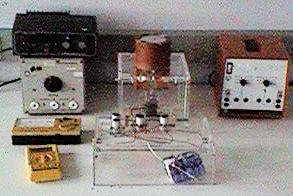
\includegraphics[scale = 0.5]{aufbau.JPG}
  	\caption[Foto der Hauptbestandteile des Versuchs]{Foto der Hauptbestandteile des Versuchs\footnotemark}
  \label{fig:aufbau}
\end{figure}
\footnotetext{Graphik wurde am 22.08.2014 von der Seite: http://www.atlas.uni-wuppertal.de/~kind/apjpg/ap1e3a.JPG entnommen}

\section{Versuchsdurchführung}


\subsection{Praktische Durchführung}

\begin{itemize}
\item	l$_{12}$:	Länge der ersten Ablenkplatten
\item	L$_{12}$:	Abstand zwischen dem Ende der Ablenkplatten bis zum Auffangschirm
\item	d$_{12}$:	Abstand zwischen den ersten Ablenkplatten
\item	l$_{34}$:	Länge der zweiten Ablenkplatten
\item	L$_{34}$:	Abstand zwischen dem Ende der Ablenkplatten bis zum Auffangschirm
\item	d$_{34}$:	Abstand zwischen den zweiten Ablenkplatten
\end{itemize}


\begin{itemize}
\item[(a)] Ablenkung im transversalen elektrischen Feld
\newline
\begin{enumerate}
\item
Messen Sie mit einem Lineal an einer Musterröhre die Abstände
L$_{12}$, l$_{12}$ und d$_{12}$
sowie L$_{34}$, l$_{34}$ und d$_{34}$ für die beiden Ablenkplattenpaare. Als Richtwerte können Sie annehmen:
l$_{12}$ = l$_{34}$ = 35$\pm$2mm. Es steht eine geöffnete Röhre zur Verfügung,
an der Sie L$_{12}$ und L$_{34}$ abschätzen können.
Da die Ablenkplatten teilweise gebogen sind (siehe Abbildung der Röhre im An-
hang), müssen Sie für den Meßwert des Plattenabstands
d$_{12}$ und d$_{34}$ eine vernünftige Abschätzung machen. Ein Wert zwischen 2 und 5 mm sollte sinnvoll sein.
\begin{figure}[htbp] 
	  \centering
	    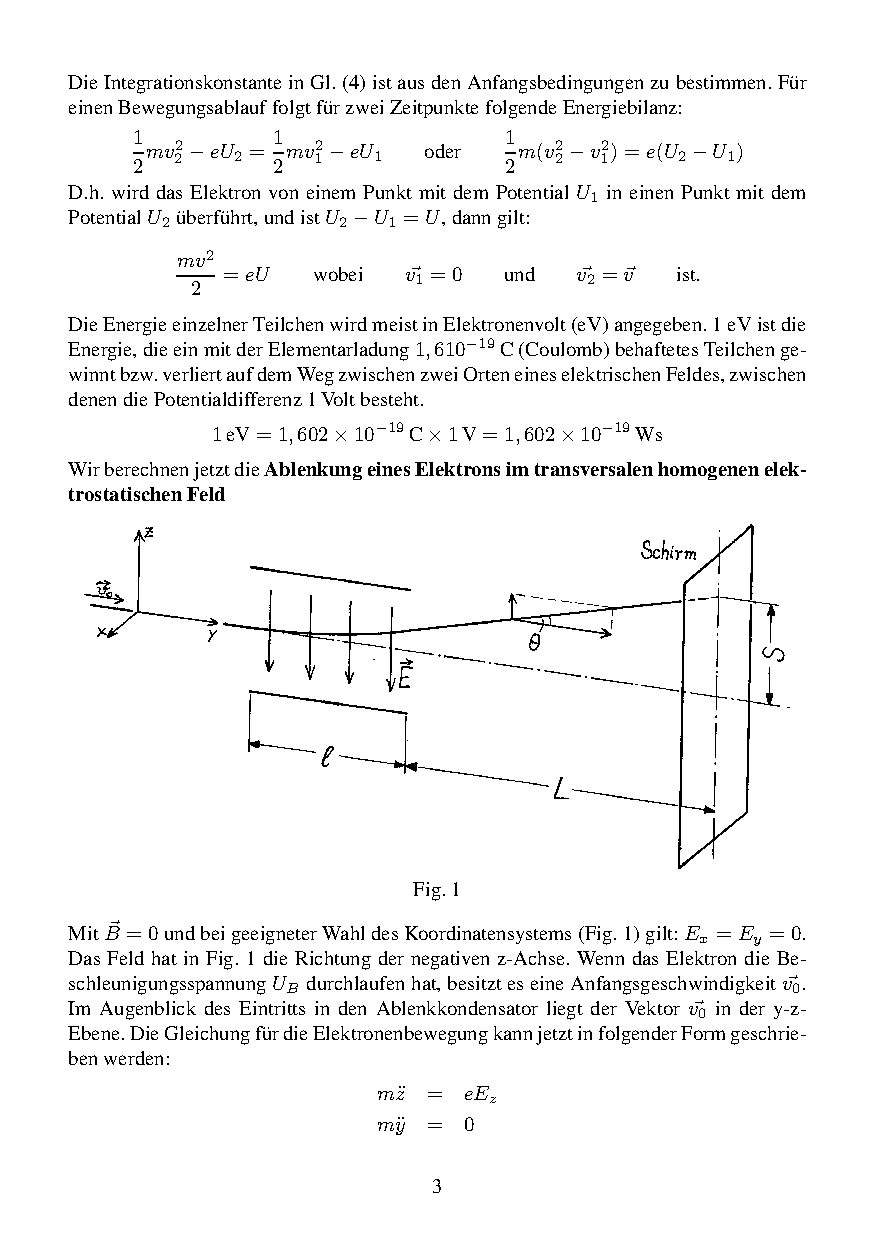
\includegraphics[trim = 1mm 61mm 1mm 85mm, clip, scale = 1]{E_ablenkung.pdf}
	  	\caption[Skizze für die Ablenkung der Elektronen durch das E-Feld]{Skizze für die Ablenkung der Elektronen durch das E-Feld\footnotemark}
	  \label{fig:E_ablenkung}
	\end{figure}
	\footnotetext{Abbildung entnommen von http://www.atlas.uni-wuppertal.de/~kind/E3.pdf Seite 3 am 22.08.2014}
\item
Setzen Sie die Oszillographenröhre mit Hilfe des Schaltplans in 
\begin{figure}[htbp] 
	  \centering
	    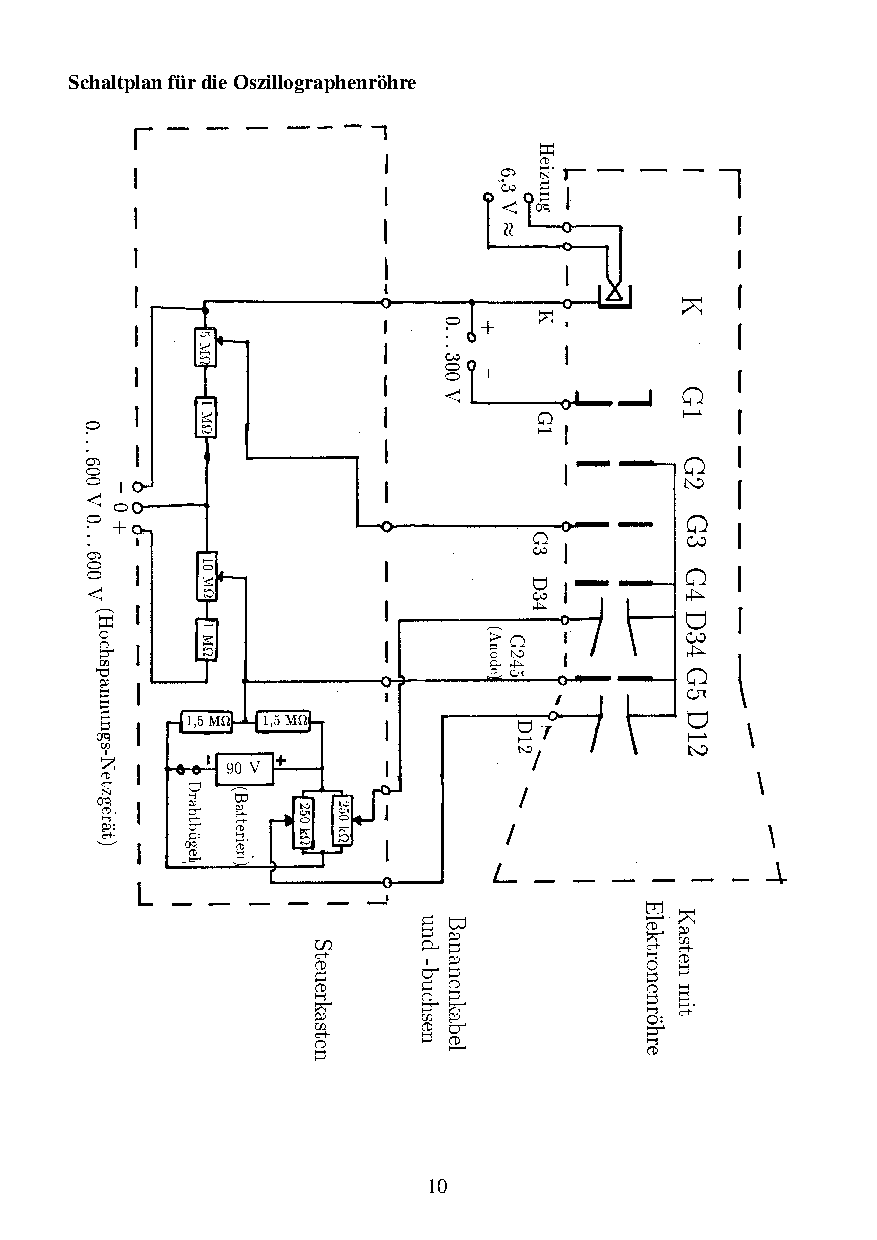
\includegraphics[trim = 1mm 17mm 1mm 17mm, clip, scale = 0.5, angle =90]{schaltskizze.pdf}
	  	\caption[Schaltskizze der Oszillographenröhre und den Schaltkasten]{Schaltskizze der Oszillographenröhre und den Schaltkasten\footnotemark}
	  \label{fig:schaltskizze}
	\end{figure}
	\newpage
	\footnotetext{Abbildung entnommen von http://www.atlas.uni-wuppertal.de/~kind/E3.pdf Seite 10 am 22.08.2014}
Betrieb und stellen Sie einen scharfen Leuchtfleck ein (U$_{D12}$ = U$_{D34}$ = 0, d.h. verbinden Sie die Anschlüsse D12 und D34 mit G245).
\item
Messen Sie für eine feste Beschleunigungsspannung U$_{B}$
die Ablenkung S$_{12}$ als
Funktion der Ablenkspannung U$_{D12}$. Tragen Sie S$_{12}$
als Funktion von U$_{D12}$ in einem Diagramm auf.
\item
Wiederholen Sie diese Messung und die graphische Darstellung mit den Ablenkplatten D34.
\item
Ändern Sie die Beschleunigungsspannung U$_B$, optimieren Sie die Fokussierung
und wiederholen Sie die Messungen 3 und 4 für zwei weitere Werte von U$_B$. Stellen Sie auch diese vier Messungen graphisch dar.
\item
Als graphische Darstellung dieser 6 Messungen aus
3, 4 und 5 erwarten Sie Ursprungsgeraden, z.B. S$_{12}$ = k$_{12}$· U$_{D12}$ (warum? Welche Ursache könnte es
haben, wenn sich keine exakte Ursprungsgerade ergibt?)
Bestimmen Sie die drei Steigungen k$_{12}$ und die drei Steigungen k$_{34}$.
Berechnen Sie für alle 6 Steigungen das Produkt U$_B\cdot$k
mit der entsprechenden
Beschleunigungsspannung. Die drei Produkte U$_B\cdot$k$_{12}$
sollten etwa gleich sein
(warum?), ebenso die drei Produkte U$_B\cdot$k$_{34}$.
\item
Berechnen Sie den Mittelwert der drei Produkte U$_B\cdot$k$_{12}$. Aus diesem Mittelwert können Sie mit den gemessenen L$_{12}$ und l$_{12}$ den Plattenabstand d$_{12}$ bestimmen (nach welcher Formel?). Vergleichen Sie den so erhaltenen Wert mit dem der direkten Messung von d$_{12}$ an der Röhre.
\item
Bestimmen Sie ebenso aus dem Mittelwert der drei Produkte U$_B\cdot$k$_{34}$ und den
gemessenen L$_{34}$ und l$_{34}$ den Plattenabstand d$_{34}$. Vergleichen Sie auch diesen Wert mit dem der direkten Messung von d$_{34}$.
\item
Diskutieren Sie die Fehler, mit denen Ihre Messungen behaftet sind.
\end{enumerate}
\item[(b)] Ablenkung im transversalen Magnetfeld
\newline

\begin{figure}[htbp] 
  \centering
    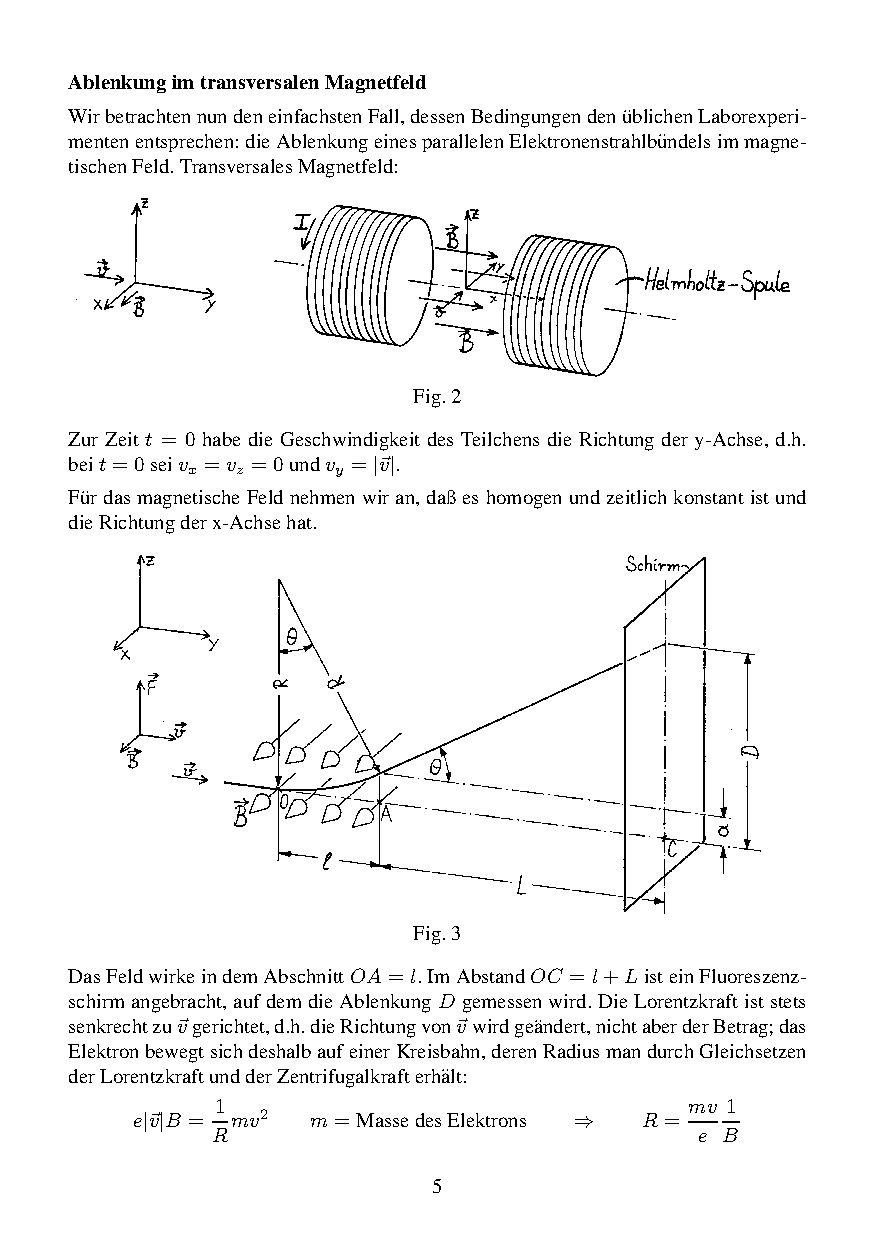
\includegraphics[trim = 1mm 55mm 1mm 91mm, clip, scale = 1]{B_ablenkung.pdf}
  	\caption[Skizze für die Ablenkung der Elektronen durch das B-Feld]{Skizze für die Ablenkung der Elektronen durch das B-Feld\footnotemark}
  \label{fig:E_ablenkung}
\end{figure}
\footnotetext{Abbildung entnommen von http://www.atlas.uni-wuppertal.de/~kind/E3.pdf Seite 5 am 22.08.2014}
Im Folgenden wird anstatt D auch S$_S$ verwendet	
\begin{enumerate}
\item[10.]
Die Röhre wird betrieben wie in (a). Die Ablenkplatten werden nicht benutzt, werden aber an die Anode (G245) angeschlossen. So wird eine statische Aufladung der Platten verhindert, die eine ungewollte Ablenkung zur Folge haben kann. Da Sie im weiteren Verlauf des Versuchs keine Ablenkspannungen
U$_{12}$ und U$_{34}$ mehr benötigen, schalten Sie bitte den 90-V-Batterieblock ab (entfernen sie den Drahtbügel
an der Seite des Steuerkastens.) Die beiden Spulen sind in Serie geschaltet, so daß sich die beiden Magnetfelder addieren. Gemessen wird die an den Spulen angelegte Spannung U$_S$. Sie ist proportional zum Strom, der durch die Spulen fließt, und damit proportional zum Magnetfeld.
\item[11.]
Messen Sie die Strahlablenkung S$_S$ als Funktion der Spulenspannung U$_S$ für feste
Beschleunigungsspannung U$_B$
und stellen Sie die Messung graphisch dar.
\item[12.]
Wiederholen Sie die Messung und graphische Darstellung für zwei andere Beschleunigungsspannungen.
\item[13.]
Sie erwarten Ursprungsgeraden S$_S$ = k$_S\cdot$U$_S$ (wieso?). Bestimmen Sie die drei Steigungen k$_S$. Berechnen Sie für jedes k$_S$
das entsprechende Produkt k$_S\cdot\sqrt{U_\text{B}}$. Vergleichen Sie
diese drei Produkte miteinander. Was erwarten Sie (warum?)
.
\end{enumerate}
\item[(c)] Erdmagnetfeld
\newline
\begin{enumerate}
\item[14.]
In (a) und (b) haben Sie beobachtet, daß bei Abwesenheit von ablenkenden Feldern die Lage des Punktes sich ändert, wenn die Beschleunigungsspannung geändert wird. Ein Grund für diesen Effekt ist das Erdmagnetfeld. Versuchen Sie, durch Markierung mit einem Fettstift auf dem Schirm eine Orientierung der Röhre zu finden, für die keine Ablenkung auftritt. Wie ist in dieser Lage die Beziehung zwischen Achsenrichtung (Elektronenstrahl) und Richtung des Magnetfeldes der Erde?
\item[15.]
Versuchen Sie jetzt, eine Orientierung zu finden, für die die Ablenkung ein Maximum hat. Bestimmen Sie die Richtung und Stärke des Magnetfeldes. Beachten Sie, daß in diesem Fall l die gesamte Länge zwischen Anode und dem Schirm ist und L = 0. Die Elektroden der jetzt verwendeten Röhren sind teilweise aus unmagnetischem Material. Für l
sollten Sie daher die Strecke mindestens von G4 zum Schirm
ansetzen (bei ferromagnetischen Ablenkplatten würde der Strahl magnetisch abgeschirmt und für l wäre der Abstand von G5 zum Schirm anzusetzen). Vergleichen Sie Ihre Bestimmung von Größe und Richtung des Erdmagnetfeldes mit Literaturwerten.
\end{enumerate}

\end{itemize}

\subsection{Theoretische Durchführung}
\begin{itemize}
\item[6.]
Der Fehler von $U \cdot k$ ist:
\begin{align}
\sigma_U = \sqrt{\left(U \sigma_k \right)^2+\left(k \sigma_U\right)^2}
\end{align}
\item[7.]
Der Mittelwert ist:
\begin{align}
M = \frac{(U_{\text{B}}k)_1+
(U_{\text{B}}k)_2+
(U_{\text{B}}k)_3}{3}
\end{align}
Der Fehler auf den Mittelwert ist:
\begin{align}
\sigma_M =\sqrt{
\left(\frac{\sigma_{(U_{\text{B}}k)_1}}{3}\right)^2+ \left(\frac{\sigma_{(U_{\text{B}}k)_2}}{3}\right)^2+
\left(\frac{\sigma_{(U_{\text{B}}k)_3}}{3}\right)^2}
\end{align}
Der Plattenabstand d berechnet sich nach der Formel:
\begin{align}
d= \frac{L l}{2 U_\text{B} k}
\end{align}
(wobei $\tan(\theta) \simeq \frac{S}{L}$ nur für $L \gg S$ gilt.)\\
Mit dem Fehler:
\begin{align}
\sigma_d = \sqrt{
\left(\frac{l}{2 U_\text{B} k}\sigma_{L}\right)^2+
\left(\frac{L}{2 U_\text{B} k}\sigma_l\right)^2+
\left(\frac{L l}{2 (U_\text{B} k)^2}\sigma_{U_\text{B} k}\right)^2}
\end{align}
\item[8.]
Berechung der Werte analog zu 7.
\item[13.]
Da die magnetische Flussdichte proportional zur Spulenspannung U$_S$ und k die Steigung der Geraden vom Plot von U$_S$ gegen S$_S$ ist, erwarten wir, dass das Produkt $k\cdot\sqrt{U_B}$ nach folgender Formel konstant ist:
\begin{align}
S_S = \frac{leB}{\sqrt{2em U_B}}(L+\frac{1}{2}l)
\end{align}
Diese Formel gilt jedoch nur für kleine Auslenkwinkel $\theta$
Der Fehler von $\sqrt{U_\text{B}} \cdot k$ ist:
\begin{align}
\sigma_{\sqrt{U_\text{B}}k} = \sqrt{
\left(\frac{k}{2\sqrt{U_\text{B}}}\sigma_{U_\text{B}}\right)^2+
\left(\sqrt{U_\text{B}}\sigma{k}\right)^2}
\end{align}
\item[15.]
Die Formel zur Berechnung des B-Feldes ist:
\begin{align}
B = \frac{2 S_\text{S}\sqrt{2 m_e U_\text{B}}}{l^2 \sqrt{e}}
\end{align}
Mit einem Fehler von:
\begin{align}
\sigma_B = \sqrt{
\left(\frac{2 \sqrt{2 m_e U_\text{B}}}{l^2 \sqrt{e}}\sigma_{S_\text{S}}\right)^2+
\left(\frac{S_\text{S}\sqrt{2 m_e}}{l^2 \sqrt{e U_\text{B}}}\sigma{U_\text{B}}\right)^2+
\left(\frac{4 S_\text{S}\sqrt{2 m_e U_\text{B}}}{l^3 \sqrt{e}}\sigma_l\right)^2
}
\end{align}
\end{itemize}

\section{Messergebnisse}



\section{Auswertung}


\section{Diskussion}


 %Werte stimmen mit den Formeln überein/nicht überein

\end{document}

